%%%%% Document Setup %%%%%%%%

\documentclass[12pt, onecolumn]{revtex4}    % Font size (12pt) and column number (one or two).

\usepackage[a4paper, left=2.5cm, right=2.5cm, top=2.5cm, bottom=2.5cm]{geometry}  % Defines paper size and margin length

\renewcommand{\baselinestretch}{1}     % Defines the line spacing

\usepackage{subcaption}

\usepackage[font=small, labelfont=bf]{caption}                      % Defines caption font size and caption title bolded
\captionsetup[figure]{justification=justified, singlelinecheck=off, font=footnotesize} 
\captionsetup{compatibility=false}

\usepackage{graphics,graphicx,epsfig,ulem}	% Makes sure all graphics works
\usepackage{amsmath} 						% Adds mathematical features for equations

\usepackage{fancyhdr}

\usepackage{textcomp}

\usepackage{tabularx}

\def\thesection{\arabic{section}}
\def\thesubsection{\alph{subsection}}

\def\bibsection{\section*{References}}        % Position reference section correctly

%%%%% Document %%%%%
\begin{document}                     

\title{Testing the Milankovitch-Croll hypothesis using $\delta^{18}$O foram data} 
\maketitle
%\thispagestyle{plain} % produces page number for front page

\vspace{-4ex}

The Milankovitch-Croll hypothesis suggests that changes in the Earth's orbit around the Sun leads to changes in the Earth's planetary climate through fluctuations in solar insolation \cite{ruddiman_climate}. We can access and view this change of climate through analysing proxy data. By using deep ocean sediment cores and Earth orbital data, we can explore the hypothesis and it's validity through performing various data analysis techniques. \\

We begin with the importance of sediment cores. Their usefulness arises from the fact that they contain a good trace for measuring the $\delta^{18}$O ratio across periods of Earth's history \cite{droxler_climate}. The change in this ratio can provide us with an indication of how the global temperature has been fluctuating across eras, this could then be linked to other climate changes such as whether the global ice volume has been increasing or decreasing. \\

Defined from laboratory experiments, for a $\sim 5^{\circ}\mathrm{C}$ temperature increase there is an $\sim 1$\textperthousand\ decrease in the $\delta^{18}$O ratio of a foram shell. As ice-sheets melt, more $^{16}$O is released into the ocean, thus reducing the ratio. Looking at Figure \ref{fig:foram_data} we can see the sediment core data for two periods from Earth's history. In the more recent age the amplitude of the $\delta^{18}$O varies more considerably than from 4 Myr to 5 Myr, suggesting that close to present times there have been longer periods of cooling due to a more dramatic shift in temperature. With a cooler climate, there would be a larger amount of ice on the planet. Comparing with the older $\delta^{18}$O data, we see that it still features the sinusoidal like trend, albeit with a smaller amplitude. This suggests that the glacial-interglacial events are a normal part of Earth's planetary climate cycle. \\

% not a fan of the above paragraph, it's a bit convoluted
% TODO discuss changes in global ice volume, particularly in the last 2-3 million years

It is then not difficult to suggest that there might be a connection between glacials-interglacials and the cyclical Earth-Sun orbital relationship. Through the analysis of such astrophysical data and paired with sediment cores we can further our investigation. \\

To start with, we can can consider the each of the separate but interlinked features, namely eccentricity, obliquity, and precession. The former describes the ellipticity of the Earth's orbit around the Sun \cite{carroll_astro}, however the effect of eccentricity $\varepsilon$ on insolation is not entirely independent as the eccentricity also depends on the orbital angle between the solstices and the position of perihelion/aphelion $\omega$. This can be summarised as $\chi= \varepsilon \sin{\omega}$, where $\chi$ is the precessional index. Finally, the obliquity is given as the value which describes the degree of tilt of the Earth's axis. \\

With these definitions in mind, we can proceed to evaluate the orbital data by applying two statistical analysis techniques. The first of which is wavelet analysis (WA), using the software package PAST3 \cite{past3} we can obtain heatmaps as shown in \ref{fig:wa_orbital_data}. Parsing the data through WA allows us to pick out the dominant frequencies in the data \\

If we are able to so that the tools can be used on the $\delta^{18}$O foram data as well. \\

The eccentricity describes how elliptical the orbit of the Earth is around the Sun \cite{carroll_astro}. From an initial wavelet analysis using the software PAST3 \cite{past3} we find that there are three wavelengths of interest. In Figure \ref{fig:wa_orbital_data}(a) and from Table \ref{table:final_results} we see that the dominant signal throughout the dataset is 401.7 ka, with 89.1 ka and 100.4 ka as two other signals present. However, the influence of eccentricity on insolation is not independent as eccentricity $\varepsilon$ depends on the angle between the solstices and the perihelion/aphelion $\omega$ on the orbit. This can be summed up to be $\chi= \varepsilon \sin{\omega}$, where $\chi$ is the precessional index. Performing a similar wavelet analysis we can see in Figure \ref{fig:wa_orbital_data}(b) that there is only one main wavelength prevalent at 21.1 ka. Finally obliquity is the third orbital feature to consider, this value represents the tilt of the Earth's axis, with Figure \ref{fig:wa_orbital_data}(c) we can find a wavelength of 39.4 ka. \\ 

Comparison with the ``true'' wavelengths, from Table \ref{table:final_results} 

\newpage

%\twocolumngrid

\bibliographystyle{unsrt}
\bibliography{practical_2}

\newpage

\section*{Appendices}
\begin{figure}[!h]
\begin{center}
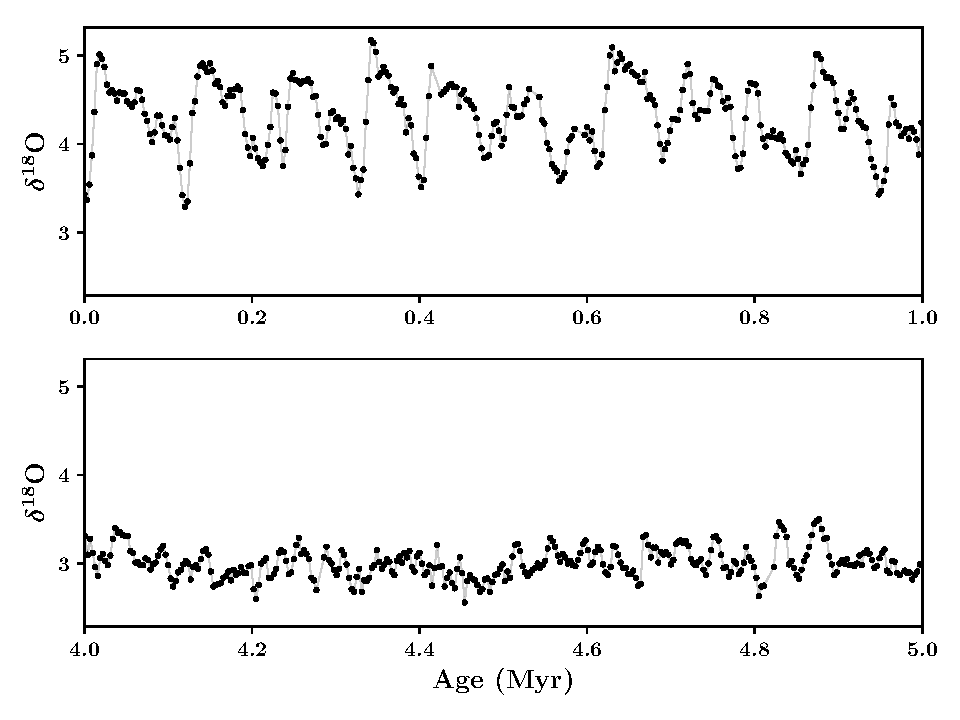
\includegraphics[width=11cm]{figures/foram_data}
\caption[]{Plots of the marine benthic foram $\delta^{18}$O data against age since the present day (the holocene). Both data sets have been taken out of a larger set which spans from 0 Myr to 6 Myr. We see that as we move closer towards the present day, the periodicity and amplitude is larger which implies that there is a more extreme temperature variation.}
\vspace{-3ex}
\label{fig:foram_data}
\end{center}
\end{figure}

\begin{figure}[!h]
\begin{center}
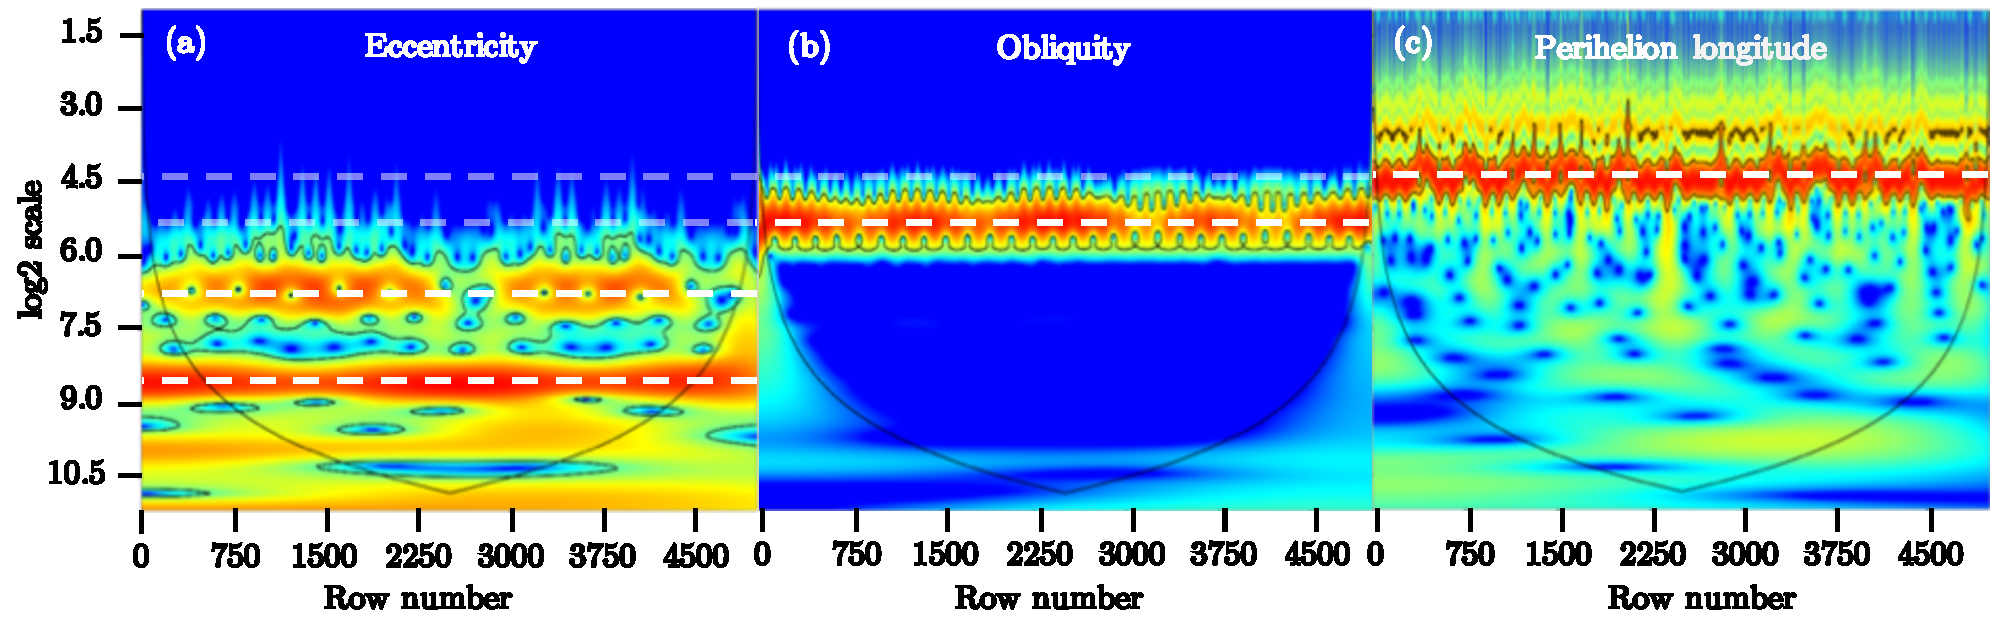
\includegraphics[width=16cm]{figures/wa_orbital_data}
\caption[]{The eccentricity, obliquity and perihelion longitude orbital data processed with the wavelet analysis tool in PAST3. The periodicities from the data can be obtained by considering the ``hottest'' areas of each of the heat maps. In Table \ref{table:final_results} we summarise the wavelengths which can be obtained from the dashed lines.}
\vspace{-3ex}
\label{fig:wa_orbital_data}
\end{center}
\end{figure}

\begin{figure}[!h]
\begin{center}
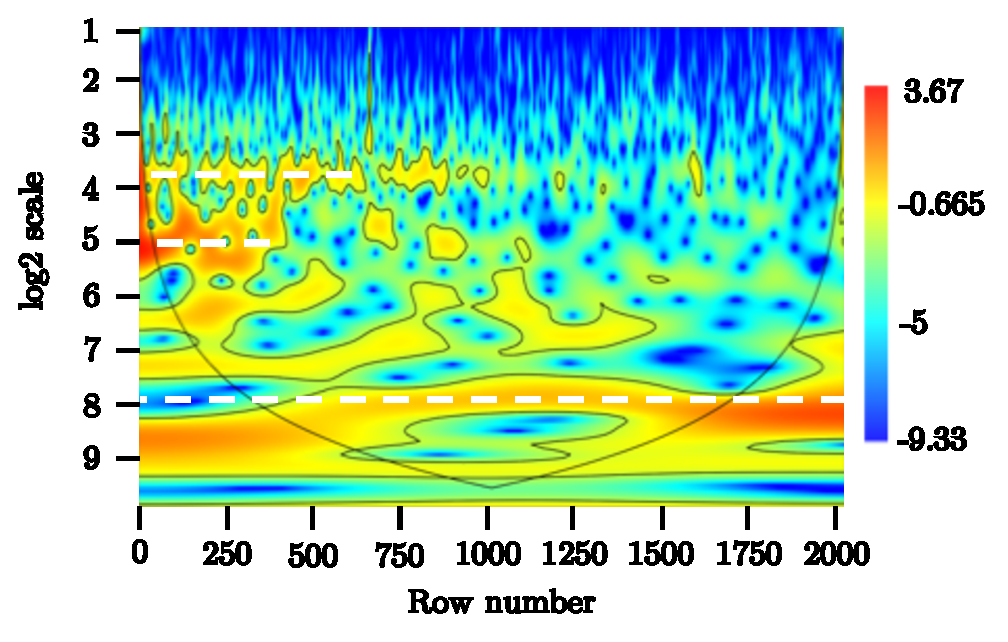
\includegraphics[width=11cm]{figures/wa_d18O.pdf}
\caption[]{Applying the PAST3 wavelet analysis tool to the $\delta^{18}$O benthic foram data we can use this as one of the possible ways to verify if the Milankovitch-Croll hypothesis is valid.}
\vspace{-3ex}
\label{fig:wa_d18o}
\end{center}
\end{figure}

\begin{figure}[!h]
\begin{center}
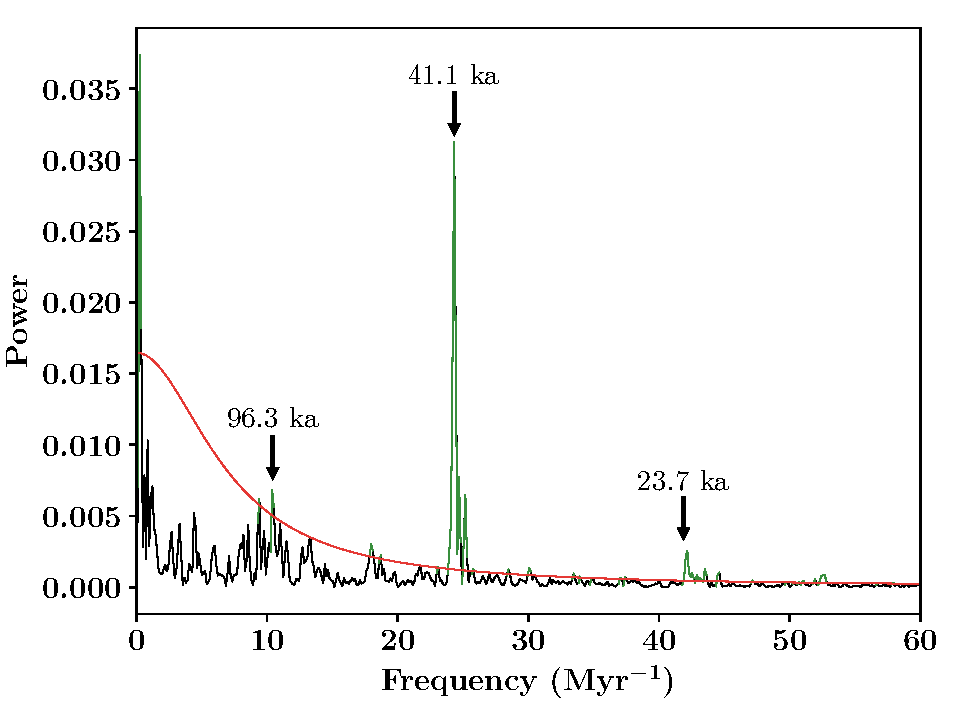
\includegraphics[width=11cm]{figures/d18O_redfit}
\caption[]{The benthic foram $\delta^{18}$O data analysed using the REDFIT spectral analysis tool in PAST3.}
\vspace{-3ex}
\label{fig:d18o_redfit}
\end{center}
\end{figure}

\begin{table}[h!]
\centering
\begin{tabular}{c@{\hskip 20pt}c@{\hskip 20pt}c@{\hskip 20pt}c} 
 \hline
  & \textbf{``True'' (ka)} &\textbf{REDFIT (ka)} & \textbf{WA (ka)} \\ [0.5ex] 
 Eccentricity & 100, 413 & 95.2, 128.2, 416.7 & 89.1, 100.4,  401.7\\
 Perihelion Longitude & 23, 100 & 23.8, 22.2 & 21.1 \\
 Obliquity & 41 & 41.7 & 39.4 \\
 $\delta^{18}$O & & 23.7, 41.1, 96.3  & 38.9, 96.0, 271.5, \\
 & & & 945.5, 1247.6 \\
 \hline
\end{tabular}
\caption{Table showing three columns of wavelength data: the approximate correct wavelengths for the periodicity of the orbital features \cite{campisano_milankovitch}, and the results of the REDFIT analysis and Wavelet Analysis (WA) on the orbital and benthic foram data.}
\vspace{-0.5em}
\label{table:final_results}
\end{table}

\end{document}